\section{Scopo e preparazione}

Si intende realizzare un'oscillatore sinusoidale a ponte di Wien con un OpAmp TL081
e osservarne il funzionamento, verificando le relazioni previste con le caratteristiche dei componenti utilizzati.
Si è dunque montato il circuito in \fig{circ}, utilizzato invariato in tutta l'esperienza; i valori misurati
per i componenti sono riportati in \tab{comp_mis}.

\begin{figure}[h]
	\centering
	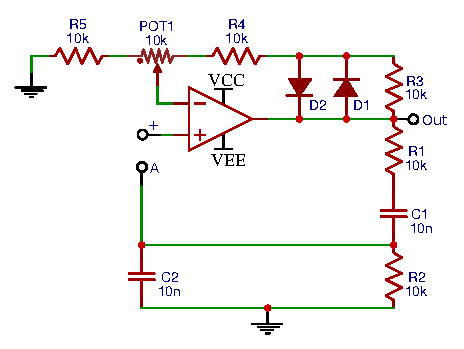
\includegraphics{circuito.pdf}
	\caption{Circuito oscillatore a ponte di Wien.}
	\label{f:circ}
\end{figure}

\begin{table}[h]
	\centering
	\begin{tabular}{ *{5}{S[table-figures-decimal=2]} *{2}{S[table-figures-decimal=1, table-figures-uncertainty=1]} }
		{$R_1$ [\si{\kohm}]} & {$R_2$ [\si{\kohm}]}	& {$R_3$ [\si{\kohm}]} & {$R_4$ [\si{\kohm}]} & {$R_5$ [\si{\kohm}]}
			& {$C_1$ [\si{\nano\farad}]} & {$C_2$ [\si{\nano\farad}]} \\
		\midrule
		9.95(9) & 9.94(9) & 9.90(9) & 9.94(9) & 9.90(9) & 10.8(5) & 10.1(4) \\
	\end{tabular}
	\caption{Misure dei componenti.}
	\label{t:comp_mis}
\end{table}

La sezione superiore del circuito, costituita dai diodi, dal potenziometro e dalle resistenze $R_{3-4-5}$,
è la rete di feedback necessaria ad utilizzare l'OpAmp come amplificatore (non invertente) rispetto all'ingresso non invertente,
mentre la sezione inferiore, costituita dal parallelo e dalla serie di resistenza e condensatore, realizza il feedback di Wien
che, riportato all'ingresso non invertente dell'OpAmp, rende il circuito un oscillatore (a patto che sia verificata la condizione di Barkhausen).

\section{Loop gain}

Intendiamo innanzitutto misuare il guadagno della rete di feedback di Wien: abbiamo dunque collegato l'ingresso
non invertente dell'OpAmp al generatore d'onda e inviato un sengale sinusoidale di ampiezza picco-picco $\approx \SI{500}{\mV}$
a varie frequenze comprese tra \SIrange[range-phrase = \text{ e }]{500}{3000}{\Hz},
misurando il segnale in uscita al punto A del circuito. Utilizzando il softare OpenChoice si sono presi i dati per ogni singola sinusoide in entrata ed uscita. Lo scopo è dunque fare un fit a tali segnali per ottenerne ampiezza,frequenza, fase ed un eventuale offset.Tale procedura è stata eseguita per ogni frequenza nel range prima considerato. Questo a permesso di trovare le ampiezze con una precisione, a patto di fattori di calibrazione, dell'ordine del 5 \textperthousand , dunque un incertezza sull'amplificazione (sempre a meno di fattori di calibrazione) dell'ordine del 7 \textperthousand.
Si è eseguito il fit del guadagno $A=\left | \frac{V_A}{V_+} \right | $ moltiplicato per il termine di feedback $\beta$ in funzione della frequenza secondo la formula $\beta A= (\frac{1}{1+\frac{R_1}{R_2}(1+\frac{\omega_s}{\omega_p}+i(\frac{\omega}{\omega_p}-\frac{\omega_s}{\omega} ))})(1 + \frac{(1-x)Pot+R_4+R_3 \paral D_1 \paral D_2}{R_5+xPot})$. Si ricorda che indicato $\omega=2 \pi f$, $\omega_p= \frac{1}{R_2C_2}$ e $\omega_s=\frac{1}{R_1C_1}$. Si è dunque fittate l'amplificazione in funzione della frequenza ottenendo la seguente curva \ref{f:lpgn} .\footnote{Il punto cerchiato in rosso è un outlier, da solo contribuiva a più di metà de $\chi^2$, dunque è stato scartato}


\begin{figure}[h]
	\centering
	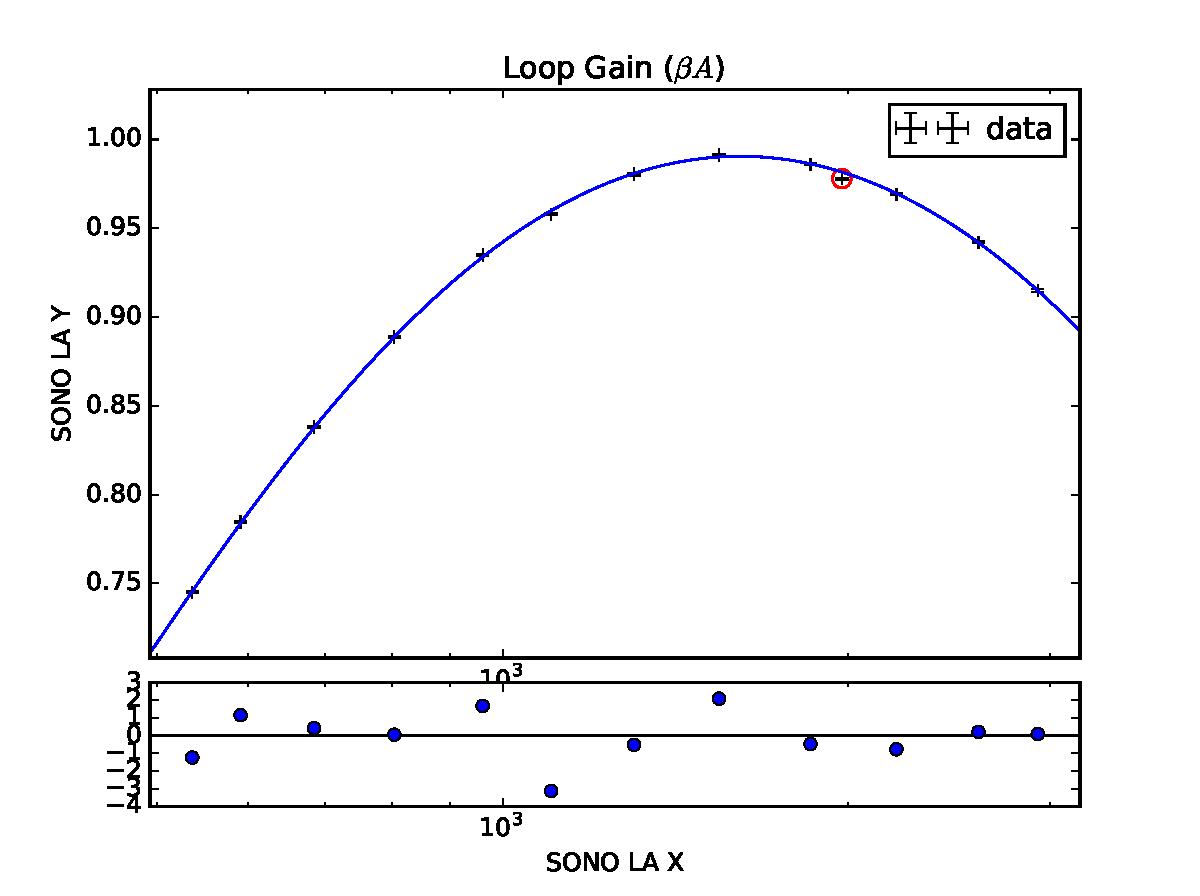
\includegraphics{loopgain.pdf}
	\caption{Loop gain e relativo fit.}
	\label{f:lpgn}
\end{figure}

Dal fit si sono ottenuti i seguenti valori:\\
$A=2.876 \pm 0.01$\\
$C_1=\SI{10.45 \pm 0.05}{nF}$ da confrontare con il valore misurato con il multimetro, di $\SI{10.81\pm 0.43}{nF}$\\
$C_2=\SI{9.44\pm 0.06}{nF}$ da confrontare con il valore misurato con il multimetro, di $\SI{10.11\pm 0.42}{nF}$\\
$corr_{C_1, C_2}=-0.92$\\
$corr_{A,C1}=-0.98$\\
$corr_{A,C2}=-0.98$\\
$\chi^2=21.26 (9 \dof, p = 0.01)$

Bisogna tenere presente che $A$ è ancora soggetto a un errore sistematico del $1.4 \%$ dovuto alle calibrazioni relative dei due canali dell'oscilloscopio. Il valore stimato di $A$ è dunque $2.876 \pm 0.04$, se non fosse che il fit non risulta statisticamente significativo, forse per una eccessiva fiducia nei parametri nella stima dei parametri.
Si nota che, in generale, il fit suggerisce una sottostima da parte del multimetro, dei  valori delle capacità.  


Stessa cosa è stata fatta per la fase. Con la stessa procedura si è ottenuto il seguente fit e i seguenti risultati:
\begin{figure}[h]
	\centering
	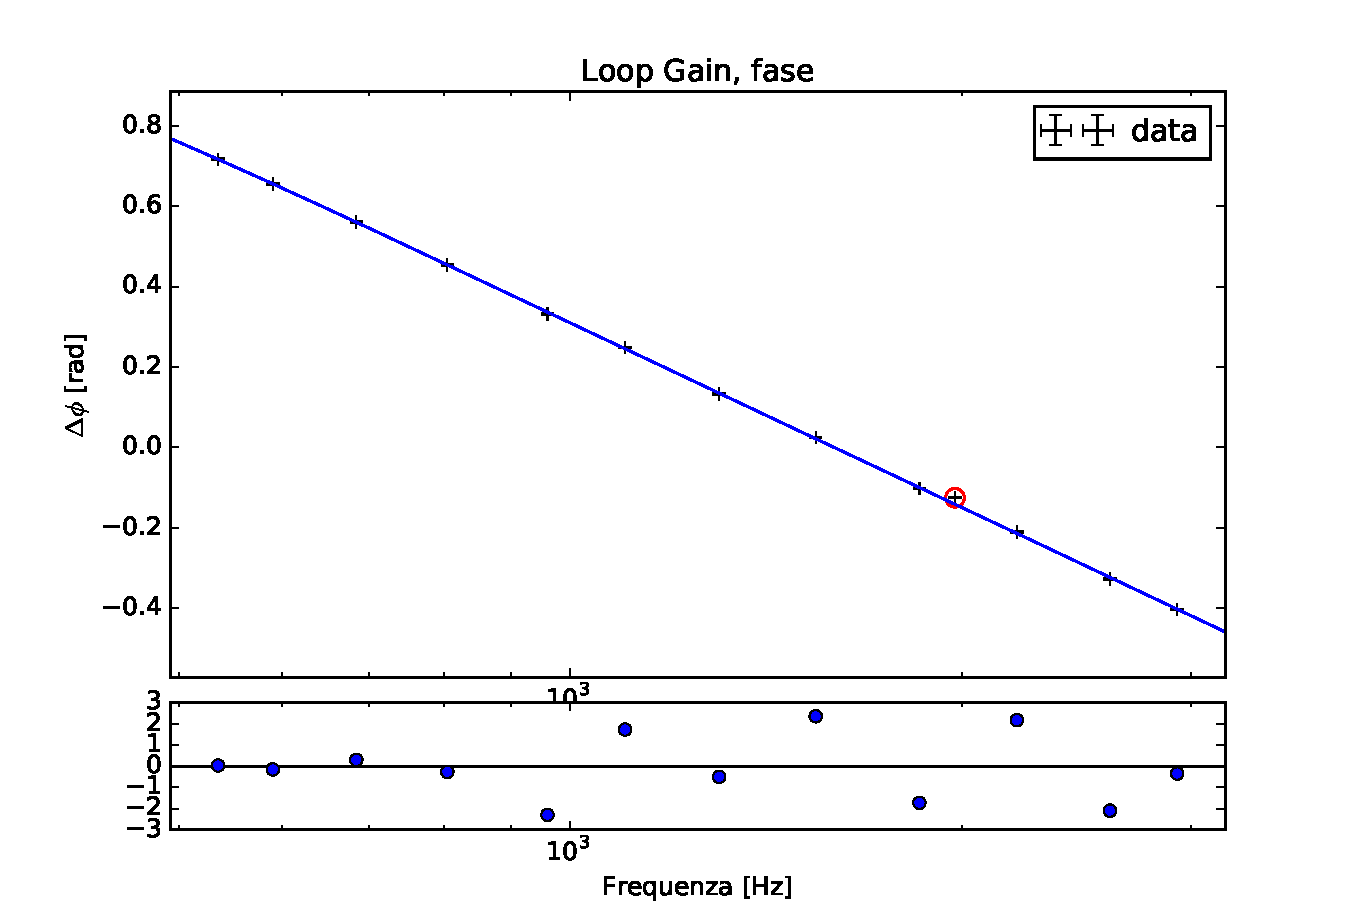
\includegraphics{phase.pdf}
	\caption{Fase introdotta dal loop e relativo fit.}
	\label{f:lpgn}
\end{figure}
$C_1=\SI{10.336 \pm 0.05}{nF}$ da confrontare con il valore misurato con il multimetro, di $\SI{10.81\pm 0.43}{nF}$\\
$C_2=\SI{9.73\pm 0.06}{nF}$ da confrontare con il valore misurato con il multimetro, di $\SI{10.11\pm 0.42}{nF}$\\
$corr_{C_1, C_2}=-0.95$\\
$\chi^2=26.45 (10 \dof, p = 0.01)$ anche questa volta non statisticamente significativo


Anche qui i valori delle capacità sono compatibili con quanto misurato con il multimetro, ma non risultano compatibili con quanto misurato con le ampiezze. Questo può essere dovuto agli errori di calibrazione su A ? Si potrebbe pensare dunque di migliorare la misura di A usando i valori delle resistenze trovate con il fit della fase per il fit dell'ampiezza (ora si fitterebbe solo il parametro A). %no, si potrebbe anche non fare, facendo così il chiq è 81!!!!
 

Dal curva di fit inoltre si ricava la frequenza per la quale la fase di $\frac{V_A}{V_+}$ è nulla, che risulta essere $\SI{1595 \pm 7}{\Hz}$\footnote{Compatibile con quanto misurato al punto 3, $\SI{1600 \pm 5}{\Hz}$}.%usando la formula di sotto, con i valori trovati in fit fase
Dall'analisi del circuito la frequenza stimata con i valori dati dal multimetro delle capacità è $f=\frac{1}{2 \pi \sqrt{R_1C_1R_2C_2}}= \SI{1.53(8)}{\kHz}$. Le due frequenze sono chiaramente compatibili. 


Variando la posizione del potenziometro si osserva che aumentando la resistenza verso $R_5$ si osserva una diminuzione dell'ampiezza del segnale in uscita , viceversa un aumento dell'ampiezza girando dalla parte opposta. Tale comportamento è analogo a quello presente in un OpAmp con feedback solo negativo .
